\documentclass[11pt,a4paper]{article}
\usepackage[top=3cm, bottom=2cm, left=2cm, right=2cm]{geometry}
\usepackage[utf8]{inputenc}
\usepackage{amsmath, amsfonts, amssymb}
\usepackage{siunitx}
\usepackage[brazil]{babel}
\usepackage{graphicx}
\usepackage[margin=10pt,font={small, it},labelfont=bf, textfont=it]{caption}
\usepackage[dvipsnames, svgnames]{xcolor}
\DeclareCaptionFont{MediumOrchid}{\color[svgnames]{MediumOrchid}}
\usepackage[pdftex]{hyperref}
\usepackage{natbib}
\bibliographystyle{plainnat}
\bibpunct{\textcolor{MediumOrchid}{\textbf{[}}}{\textcolor{MediumOrchid}{\textbf{]}}}{,}{s}{}{}
\usepackage{color}
\usepackage{footnote}
\usepackage{setspace}
\usepackage{booktabs}
\usepackage{multirow}
\usepackage{subfigure}
\usepackage{fancyhdr}
\usepackage{leading}
\usepackage{indentfirst}
\usepackage{wrapfig}
\usepackage{mdframed}
\usepackage{etoolbox}
\usepackage[version=4]{mhchem}
\usepackage{enumitem}
\usepackage{caption}
\usepackage{titlesec}
\usepackage{tcolorbox}
\usepackage{tikz}
\usepackage{LobsterTwo}
\usepackage[T1]{fontenc}
\usepackage{fontspec}
\usepackage{txfonts}
\usepackage[bottom]{footmisc}
\tcbuselibrary{skins,breakable}
\sisetup{output-decimal-marker={.}}

\makeatletter
\def\footnoterule{\kern-3pt\color{MediumOrchid}\hrule\@width0.6\textwidth height 0.8pt\kern2.6pt}
\makeatother

\renewcommand{\footnotelayout}{\itshape\color{MediumOrchid}}

\AtBeginEnvironment{equation}{\fontsize{13}{16}\selectfont}


\titleformat{\section}{\LobsterTwo\huge\color{CarnationPink}}{\thesection.}{1em}{}
\titleformat{\subsection}{\LobsterTwo\huge\color{CarnationPink}}{\thesubsection}{1em}{}
\titleformat{\subsubsection}{\bf\LobsterTwo\Large\color{MediumOrchid}}{\thesubsubsection}{1em}{}


\DeclareCaptionLabelFormat{figuras}{\textcolor{DarkTurquoise}{Figura \arabic{figure}}}
\captionsetup[figure]{labelformat=figuras}

\makeatletter
\renewcommand\tagform@[1]{\maketag@@@{\color{CarnationPink}(#1)}}
\makeatother

\renewcommand{\theequation}{Eq. \arabic{equation}}
\renewcommand{\thefigure}{Fig. \arabic{figure}}
\renewcommand{\thesection}{\textcolor{CarnationPink}{\arabic{section}}}

\setlist[itemize]{label=\textcolor{CarnationPink}{$\blacksquare$}}

\setlist[enumerate]{label=\textcolor{CarnationPink}{\arabic*.}, align=left, leftmargin=1.5cm}


\newcounter{exemplo}

\NewDocumentEnvironment{exemplo}{ O{} }{%
\allowbreak
\setlength{\parindent}{0pt}
  \begin{mdframed}[
  leftline=true,
  topline=false,
  rightline=false,
  bottomline=false,
  linewidth=2pt,
  linecolor=CarnationPink,
  frametitlerule=false,
  frametitlefont=\LobsterTwo\large\color{CarnationPink},
  frametitle={\color{CarnationPink}\LobsterTwo\large #1},
  ]
}{%
  \end{mdframed}
}

\setlength{\fboxsep}{5pt}
\setlength{\fboxrule}{1.5pt}
\usepackage{float}
\renewcommand{\thefootnote}{\alph{footnote}}
\usepackage{url}
\hypersetup{
	colorlinks=true,
	linkcolor=DarkTurquoise,
	filecolor=DarkTurquoise,      
	urlcolor=DarkTurquoise,
	citecolor=DarkTurquoise,
	pdftitle={Especialista em Física da Radioterapia}
}
\pagestyle{fancy}
\fancyhf{}
\renewcommand{\headrulewidth}{0pt}
\rfoot{\color{DarkTurquoise}\thepage \\ \LobsterTwo{\small\textcolor{CarnationPink}{@defDalila}}}

\title{\LobsterTwo\Huge{Radiobiologia}}
\author{\LobsterTwo\Large{Mecanismos De Morte Celular e Ensaios de Sobrevivência}\nocite{*}}
\date{\LobsterTwo\textit{Dalila Mendonça}}
\begin{document}
	\maketitle



\section{Morte Celular}

	A \textcolor{DarkTurquoise}{\textbf{\textit{morte celular}}} na radiobiologia é definida como a \textcolor{MediumOrchid}{\textbf{\textit{perda da capacidade clonogênica}}} de uma célula. A definição de morte celular é extremamente importante ao abordar a erradicação de tumores e a inibição do seu crescimento.
	
	Quando as células tumorais perdem a capacidade de se reproduzir, elas deixam de ser \textcolor{MediumOrchid}{\textbf{\textit{viáveis}}} clonogenicamente, ou seja, não conseguem mais formar colônias de células viáveis. Isso é um aspecto crucial no tratamento de câncer, pois a capacidade de um tumor se reproduzir e crescer é fundamental para sua sobrevivência e propagação.

	Além disso, a \textcolor{MediumOrchid}{\textbf{\textit{perda da integridade reprodutiva}}} também é relevante para \textcolor{MediumOrchid}{\textbf{\textit{tecidos normais}}} que se dividem rapidamente, como o intestino e a medula óssea. Esses tecidos normais em rápida divisão são sensíveis à radioterapia ou quimioterapia, que visam danificar o DNA das células em passando por divisão, prejudicando sua capacidade de se replicar. A perda da capacidade de se reproduzir nessas células normais pode ter \textcolor{MediumOrchid}{\textbf{\textit{efeitos colaterais indesejados}}}, como danos ao revestimento do intestino ou supressão da produção de células sanguíneas na medula óssea.

	Por outro lado, o \textcolor{MediumOrchid}{\textbf{\textit{a definição de morte celular não é tão relevante para tecidos normais altamente diferenciados}}}, como os nervos e músculos. Esses tecidos já são considerados "mortos" de acordo com essa definição, pois \textcolor{MediumOrchid}{\textbf{\textit{não possuem capacidade de divisão celular significativa}}}. Esses tecidos têm células altamente especializadas e seu papel principal é a condução de sinais elétricos (no caso dos nervos) ou a contração muscular (no caso dos músculos), e não a proliferação celular.

	\textcolor{MediumOrchid}{\textbf{\textit{Células com extensos danos no DNA podem continuar a se dividir por algumas vezes após o dano antes de chegarem a um ponto em que não conseguem mais se dividir}}}. Nesse ponto, a célula é considerada "morta" reprodutivamente, ou seja, ela perdeu a capacidade de se reproduzir e gerar novas células. Quando uma célula se torna reprodutivamente morta, ela se torna \textcolor{MediumOrchid}{\textbf{\textit{não clonogênica}}}. Isso significa que a célula não é capaz de formar uma colônia em um ambiente de cultura in vitro, onde as células são cultivadas em laboratório. Além disso, a célula também não pode reestabelecer um clone ou um tumor em um ambiente in vivo, ou seja, no organismo vivo.

\subsection*{Mecanismos de Morte Celular Após a Irradiação}

	\begin{itemize}[label=\textcolor{CarnationPink}{$\blacktriangleright$}]
		\item \textcolor{DarkTurquoise}{\LobsterTwo\Large\textbf{Necrose:}}
		
		A necrose é uma forma \textcolor{MediumOrchid}{\textbf{\textit{``passiva''}}} não programada de morte celular geralmente desencadeada por danos extensos e irreversíveis às células.

		\textcolor{MediumOrchid}{$(i)$} A necrose geralmente é desencadeada por uma lesão  grave que excede a capacidade das células de se adaptarem e sobreviverem. Isso pode incluir falta de oxigênio, toxinas, infecção, traumas ou temperaturas extremas. \textcolor{MediumOrchid}{$(ii)$} A lesão causa disrupção na membrana plasmática da célula, resultando em vazamento de conteúdo intracelular. Isso ocorre devido ao aumento da permeabilidade da membrana, o que leva à perda do equilíbrio iônico e acúmulo de íons e substâncias intracelulares no ambiente extracelular. \textcolor{MediumOrchid}{$(iii)$} A ruptura da célula e a liberação de substâncias intracelulares podem desencadear uma resposta inflamatória. Os mediadores inflamatórios, como citocinas e quimiocinas, são liberados, atraindo células inflamatórias, como neutrófilos e macrófagos, para a área afetada. \textcolor{MediumOrchid}{$(iv)$} A lesão e a ruptura da membrana podem levar ao influxo de água e sais minerais para dentro da célula, resultando em um inchaço celular chamado edema. Esse inchaço ocorre devido a distúrbios no equilíbrio osmótico e na função das bombas de íons da célula. \textcolor{MediumOrchid}{$(v)$} A necrose geralmente leva à ruptura do núcleo da célula, resultando na dispersão do material genético no citoplasma. Esse processo é chamado de cariorrexe. \textcolor{MediumOrchid}{$(vi)$}  Durante a necrose, várias enzimas e outras substâncias intracelulares são liberadas no ambiente extracelular, incluindo enzimas lisossômicas, proteínas citoplasmáticas e conteúdo mitocondrial. Essas substâncias podem ser tóxicas para as células vizinhas e atraentes para células inflamatórias, ampliando a resposta inflamatória. \textcolor{MediumOrchid}{$(vii)$} Após a necrose, o corpo inicia o processo de reparo, formando tecido de granulação\footnote{Tecido de granulação é um tipo de tecido de reparação que se forma durante o processo de cicatrização de feridas ou lesões}. Isso envolve a proliferação de células e vasos sanguíneos a partir do tecido saudável adjacente para preencher a área lesionada.
		

		\item \textcolor{DarkTurquoise}{\LobsterTwo\Large\textbf{Apoptose:}}
		
		É a \textcolor{MediumOrchid}{\textbf{\textit{forma mais comum de morte celular programada}}}. Também é conhecida como morte de interfase para ser diferenciada da morte mitótica. Na apoptose a célula sofre uma série de mudanças ordenadas e degenerativas.

		\textcolor{MediumOrchid}{$(i)$} A apoptose é desencadeada por uma variedade de estímulos, como sinais celulares, danos ao DNA, estresse celular, falta de nutrientes, entre outros. Esses estímulos ativam vias de sinalização que levam à ativação de proteases específicas chamadas caspases, que são as principais mediadoras da apoptose. \textcolor{MediumOrchid}{$(ii)$} Um dos primeiros sinais visíveis da apoptose é a condensação do material genético no núcleo da célula. O DNA se fragmenta e se compacta, formando estruturas características chamadas corpos apoptóticos. \textcolor{MediumOrchid}{$(iii)$} O DNA da célula em apoptose sofre fragmentação em múltiplos fragmentos de tamanho característico. Esses fragmentos são resultantes da ativação de endonucleases, enzimas responsáveis pela quebra do DNA. \textcolor{MediumOrchid}{$(iv)$}  Durante a apoptose, a membrana plasmática sofre mudanças estruturais. Moléculas lipídicas específicas, chamadas fosfatidilserina, são expostas na face externa da membrana, sinalizando para células vizinhas e células fagocitárias que devem remover a célula apoptótica. \textcolor{MediumOrchid}{$(v)$}  A célula apoptótica se retrai e se fragmenta em pequenos corpos apoptóticos. Esses corpos contêm o material celular compactado e fragmentado, bem como organelas celulares. \textcolor{MediumOrchid}{$(vi)$}  Os corpos apoptóticos são reconhecidos e englobados por células vizinhas ou por células especializadas no sistema imunológico, como macrófagos. Esse processo de fagocitose permite a remoção eficiente dos restos celulares sem causar inflamação ou danos ao tecido. \textcolor{MediumOrchid}{$(vii)$} Ao contrário da necrose, a apoptose ocorre sem desencadear uma resposta inflamatória significativa. Isso ocorre porque a célula apoptótica é rapidamente fagocitada e removida, evitando a liberação de substâncias inflamatórias.

		A apoptose é parte importante do desenvolvimento embrionário normal. O desaparecimento da teia interdigital nas mãos de alguns mamíferos e a regressão das caudas dos girinos são exemplos de apoptose. 

		A apoptose ocorre em resposta à radiação em algumas, mas não em todas as células. Células muito \textcolor{MediumOrchid}{\textbf{\textit{radiossensíveis}}}, como linfócitos normais, linfoma e células de neuroblastoma, \textcolor{MediumOrchid}{\textbf{\textit{têm muita apoptose}}}. Células tumorais muito \textcolor{MediumOrchid}{\textbf{\textit{radiorresistentes}}}, como melanoma e glioblastoma, \textcolor{MediumOrchid}{\textbf{\textit{não apresentam apoptose significativa}}}.


		\item \textcolor{DarkTurquoise}{\LobsterTwo\Large\textbf{Autofagia:}}
		
		Na autofagia \textcolor{MediumOrchid}{\textbf{\textit{a célula degrada seus próprios componentes utilizando os lisossomos}}}. Normalmente ocorre em resposta à privação de nutrientes; no entanto, muitos cânceres humanos, incluindo adenocarcinomas pancreáticos, dependem da reciclagem autofágica de componentes celulares para sustentar o crescimento das células tumorais.

		Muitas vezes, a autofagia é uma parte normal do crescimento/desenvolvimento celular e permite que as células encontrem um equilíbrio entre síntese, degradação e reutilização de componentes celulares, principalmente em resposta à inanição celular\footnote{Inanição celular se refere a uma condição na qual as células não recebem nutrientes adequados para sobreviver e funcionar corretamente.}.

		A degradação de componentes celulares pelo lisossomo é desencadeada por proteínas codificadas por genes relacionados à autofagia, ou ATG, notadamente Atg8 e Atg6 (ou LC3 e Beclin-1, respectivamente, em células de mamíferos). Este processo envolve a formação do autofagossomo, que sequestra uma organela ou material e depois se funde com um lisossomo, onde ocorre a degradação do conteúdo do autofagossomo. A autofagia pode ser induzida por inibição de mTOR, ativação de PI3K, ativação mitocondrial de ERK ou ativação de JNK.

		A cloroquina e a hidroxicloroquina, que têm sido usadas como tratamento e profilaxia para a malária, demonstraram inibir a autofagia em cânceres humanos.

		\item \textcolor{DarkTurquoise}{\LobsterTwo\Large\textbf{Catástrofe Mitótica:}}
		
		A catástrofe mitótica (ou morte mitótica) \textcolor{MediumOrchid}{\textbf{\textit{ocorre quando as células são incapazes de segregar adequadamente seus cromossomos durante a mitose}}}. A morte celular ocorre devido a danos maciços no DNA. As células geralmente não conseguem completar a citocinese e geralmente se tornam células multinucleadas “gigantes” que contêm vários micronúcleos.

		A catástrofe mitótica é causada por aberrações letais do DNA, que são causadas por quebras na fita dupla do DNA pela irradiação. \textcolor{MediumOrchid}{\textbf{\textit{A aberração do DNA não é letal até que a célula tente a mitose}}}, então há um atraso de tempo entre a irradiação e a catástrofe mitótica. Este processo é dependente do tipo de célula e é por isso que leva de dias a semanas para um tumor regredir após a irradiação.
		
		\item \textcolor{DarkTurquoise}{\LobsterTwo\Large\textbf{Senescência:}}
		
		É definida como a \textcolor{MediumOrchid}{\textbf{\textit{cessação do ciclo celular}}}. Neste processo, as células permanecem intactas, mas tornam-se incapazes de se dividir devido a danos no DNA. Isso as torna “reprodutivamente mortas”, embora as células ainda estejam lá. A senescência é uma \textcolor{MediumOrchid}{\textbf{\textit{parte normal do envelhecimento celula}}}r, mas também pode ocorrer em resposta a lesões, incluindo aquelas induzidas pela radiação. As proteínas p16 e $\beta$-galactosidase são marcadores moleculares de senescência.

		\item \textcolor{DarkTurquoise}{\LobsterTwo\Large\textbf{Necroptose:}}
		
		A necroptose é outra \textcolor{MediumOrchid}{\textbf{\textit{forma regulada de morte celular}}} porém independente de caspase. A morte celular é executada por “proteínas quinases de interação com o receptor” RIP1 e RIP3, MLKL. A formação do necrossoma (um complexo de RIP1, RIP3 e MLKL) faz a mediação de eventos, como uma explosão de espécies reativas de oxigênio (ROS), e a permeabilização da membrana plasmática. A RIP1 deve fosforilar e ativar RIP3, e a RIP3 deve fosforilar a MLKL para formar o trímero. O trímero MLKL se transloca para a membrana plasmática, causando permeabilização da membrana plasmática. Este é um mecanismo de execução chave. A necroptose pode ser inibida por agentes que atuam em RIP1, RIP3 e MLKL.

		\item \textcolor{DarkTurquoise}{\LobsterTwo\Large\textbf{Anoikis:}}
		
		É uma \textcolor{MediumOrchid}{\textbf{\textit{forma alternativa de morte celular programada}}}. A Anoikis é uma morte celular programada que ocorre quando as células são colocadas em um órgão ou tecido desconhecido. As células cancerígenas devem superar anoikis para ocorrer metástases. A proteína BIM-EL está associada a este processo. Esse processo facilita a liberação do citocromo C da mitocôndria, ativando por sua vez caspases e desencadeando a fragmentação do DNA semelhante ao que é observado durante a apoptose.
	\end{itemize}


\subsection*{Reações Teciduais após a Irradiação}

	\begin{itemize}[label=\textcolor{CarnationPink}{$\star$}]
		\item A \textcolor{DarkTurquoise}{\textbf{Apoptose}} geralmente começa dentro de \textcolor{MediumOrchid}{\textbf{\textit{6–24 h}}} após a irradiação; no entanto, também foi observada apoptose retardada (vários dias), e alterações apoptóticas iniciais podem ser observadas mais cedo em algumas linhagens celulares, dependendo dos estímulos e da dose. Os corpos apoptóticos são rapidamente degradados pelas células espectadoras, então eles desaparecem rapidamente.
		\item A \textcolor{DarkTurquoise}{\textbf{Catástrofe mitótica}} geralmente ocorre dentro de \textcolor{MediumOrchid}{\textbf{\textit{um a dois ciclos celulares}}} (15 h a 2 semanas em células ciclando ativamente).
		\item A \textcolor{DarkTurquoise}{\textbf{Necrose}} pode ser observada por \textcolor{MediumOrchid}{\textbf{\textit{dias a um pequeno número de semanas}}} após a irradiação. Em doses muito altas, pode ocorrer dentro de minutos a horas após a irradiação.
		\item As \textcolor{DarkTurquoise}{\textbf{Respostas tardias}} são caracterizadas por alterações que ocorrem no tecido irradiado após \textcolor{MediumOrchid}{\textbf{\textit{meses ou anos}}} após a exposição à radiação. Essas alterações podem não estar diretamente ligadas à morte celular, sendo as principais respostas tardias a Fibrose, alterações microvasculares, inflamação crônica e a diminuição da cicatrização de feridas.
	\end{itemize}

\section{Sobrevivência Das Células Após a Irradiação}

\subsection*{Radiossensibilidade}

	A radiossensibilidade depende de três fatores principais: \textcolor{MediumOrchid}{\textbf{\textit{conteúdo do DNA (ou tamanho do “alvo”), mecanismos de reparo e mecanismo de morte}}}. Quanto mais DNA existir em uma célula, mais fácil a radiação atingir uma dessas moléculas então é maior a sensibilidade dessa célula. Quando mais a célula é eficiente em reparo, menor a sua radiossensibilidade; e quando mais propensa a apoptose, mais a célula é radiossensível.

\subsubsection*{Células de Mamíferos}

	As células de mamíferos são \textcolor{MediumOrchid}{\textbf{\textit{altamente radiossensíveis}}} porque têm muito DNA e podem sofrer apoptose. $\sim$2 Gy pode matar aproximadamente metade das células de mamíferos, $\sim$70 Gy entregues em frações de 2 Gy podem esterilizar um tumor.

	A \textcolor{MediumOrchid}{\textbf{\textit{sobrevivência celular}}} geralmente \textcolor{MediumOrchid}{\textbf{\textit{diminui}}} à medida que o \textcolor{MediumOrchid}{\textbf{\textit{tamanho da fração (aumento da dose por fração) e a taxa de dose aumentam}}}. Isso se deve à diminuição da oportunidade para as células repararem os danos no DNA. As \textcolor{MediumOrchid}{\textbf{\textit{células que não se dividem são as mais radiorresistentes, enquanto as células que se dividem rapidamente com apoptose ativa são altamente radiossensíveis}}}.

\subsubsection*{Bactérias}

	Leveduras e bactérias são muito mais \textcolor{MediumOrchid}{\textbf{\textit{resistentes}}}, devido ao conteúdo de DNA muito menor (menor tamanho do alvo). $\sim$ 10s a 100s de Gy matarão metade das bactérias e leveduras. Um irradiador de processamento de alimentos pode fornecer até 20.000 Gy para esterilizar bactérias. 

\subsubsection*{Vírus}

	Os vírus são \textcolor{MediumOrchid}{\textbf{\textit{extremamente radiorresistentes}}} porque têm muito pouco DNA (e, portanto, têm um tamanho de alvo menor) em comparação com uma célula eucariótica. A dose letal para vírus está na faixa kGy.

\section{Ensaios de Sobrevivência}

	Existem duas abordagens diferentes utilizadas para avaliar a sobrevivência celular: Os ensaios in vitro e os ensaios in vivo.

	\begin{itemize}[label=\textcolor{CarnationPink}{$\blacktriangleright$}]
		\item Os \textcolor{DarkTurquoise}{\LobsterTwo\textbf{ensaios in vitro}} são conduzidos em um \textcolor{MediumOrchid}{\textbf{\textit{ambiente controlado em laboratório}}}, utilizando células isoladas em cultura. Nesse tipo de ensaio, as células são expostas a diferentes condições experimentais, como exposição a drogas, radiação, estresse oxidativo, entre outros; e a viabilidade celular é medida por meio de ensaios de citotoxicidade ou apoptose. As principais características de um ensaio in vitro são:
		
		\begin{itemize}[label=\textcolor{CarnationPink}{$\star$}]
			\item \textcolor{DarkTurquoise}{\textbf{Controle experimental:}} Os ensaios in vitro permitem um \textcolor{MediumOrchid}{\textbf{\textit{controle mais preciso das condições experimentais}}}, como concentração de substâncias químicas, tempo de exposição e ambiente de cultura das células.
			\item \textcolor{DarkTurquoise}{\textbf{Menor custo e tempo:}} Os ensaios in vitro geralmente são mais rápidos e menos dispendiosos em comparação com os ensaios in vivo, pois não envolvem animais vivos.
			\item \textcolor{DarkTurquoise}{\textbf{Limitações na fisiologia celular:}} As células cultivadas em laboratório \textcolor{MediumOrchid}{\textbf{\textit{podem não refletir completamente o ambiente complexo e interações celulares presentes no organismo vivo}}}.
			\item \textcolor{DarkTurquoise}{\textbf{Falta de interações sistêmicas:}} Os ensaios in vitro \textcolor{MediumOrchid}{\textbf{\textit{não podem avaliar o efeito de fatores sistêmicos}}}, como o sistema imunológico, vasculatura e outras células presentes no organismo. \textcolor{MediumOrchid}{\textbf{\textit{Não é possível medir os efeitos tardios}}}.
		\end{itemize}
		
		\item Os \textcolor{DarkTurquoise}{\LobsterTwo\textbf{ensaios in vivo}} são realizados em organismos vivos, como animais de laboratório. Nesses ensaios, as células são implantadas ou administradas nos animais, e a sobrevivência celular é avaliada em um contexto fisiológico mais complexo. As principais características dos ensaios in vivo são:
		\begin{itemize}[label=\textcolor{CarnationPink}{$\star$}]
			\item \textcolor{DarkTurquoise}{\textbf{Fisiologia mais próxima da realidade:}} Os ensaios in vivo permitem avaliar as células em um ambiente mais próximo do que ocorre no organismo vivo, incluindo interações com outros tipos de células, tecidos e sistemas. Pode medir os efeitos iniciais e tardios se esperar o tempo suficiente.
			\item \textcolor{DarkTurquoise}{\textbf{Resposta imunológica:}} Os ensaios in vivo podem fornecer informações sobre a \textcolor{MediumOrchid}{\textbf{\textit{resposta imunológica}}} às células transplantadas ou tratamentos.
			\item \textcolor{DarkTurquoise}{\textbf{Complexidade e custo:}} Os ensaios in vivo são mais complexos, exigem um maior número de recursos, tempo e expertise, além de envolverem o uso de animais vivos, o que levanta questões éticas.
			\item \textcolor{DarkTurquoise}{\textbf{Dificuldade de controle experimental:}} Alguns fatores experimentais, como a dosagem precisa e a interação complexa com outros sistemas biológicos, podem ser difíceis de controlar nos ensaios in vivo. Além disso as células animais têm tolerâncias diferentes para radiação e quimioterapia.
		\end{itemize}
	\end{itemize}


\subsection*{Ensaio de Sobrevivência Clonogênica In Vitro}

	A \textcolor{DarkTurquoise}{\textbf{sobrevivência clonogênica}} é definida pela \textcolor{MediumOrchid}{\textbf{\textit{capacidade de formar colônias}}}. O ensaio de sobrevivência clonogênica in vitro é um método utilizado para avaliar a capacidade das células de formar \textcolor{MediumOrchid}{\textbf{\textit{colônias viáveis}}} após um tratamento ou exposição a um agente de interesse. Esse ensaio é especialmente útil para medir a capacidade de sobrevivência e proliferação de células-tronco, células progenitoras ou células tumorais. Um esquema ensaio in vitro é exemplificado na \ref{fig:fracaoDeSobrevivencia}.

	\begin{figure}[h]
		\centering
		\fcolorbox{DarkTurquoise}{white}{%
			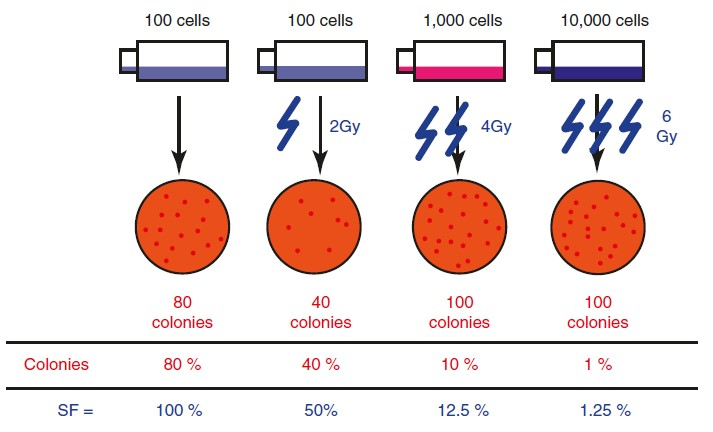
\includegraphics[width=0.8\textwidth]{Imagens/fracaoDeSobrevivencia.jpg}
		}%
		\caption{O ensaio de sobrevivência clonogênica. A fração de sobrevivência pode ser calculada dividindo a porcentagem de colônias formadas pela eficiência de formação de colônias (porcentagem de colônias formadas sem irradiação)}
		\label{fig:fracaoDeSobrevivencia}
	\end{figure}

	O ensaio de sobrevivência clonogênica in vitro é realizado da seguinte maneira:

	\begin{enumerate}[label=\textcolor{CarnationPink}{\arabic*${}^\circ $}]
		\item \textcolor{DarkTurquoise}{\textbf{Preparação das células:}} As células de interesse são isoladas e cultivadas em placas de cultura devidamente tratadas. A densidade celular é ajustada para permitir o crescimento e formação de colônias.
		\item \textcolor{DarkTurquoise}{\textbf{Tratamento ou exposição:}} As células são tratadas ou expostas a um agente ou condição de interesse. Isso pode incluir radiação ionizante, agentes quimioterápicos, drogas experimentais, entre outros.
		\item \textcolor{DarkTurquoise}{\textbf{Incubação:}} Após o tratamento, as células são incubadas em condições adequadas de cultura por um período de tempo definido. Durante essa fase, as células viáveis podem formar colônias.
		\item \textcolor{DarkTurquoise}{\textbf{Fixação e coloração:}} As células são fixadas e coradas para facilitar a visualização das colônias formadas. Isso pode ser feito utilizando corantes como o cristal violeta.
		\item \textcolor{DarkTurquoise}{\textbf{Contagem de colônias:}} As colônias são contadas manualmente ou com o auxílio de um sistema automatizado. A definição de uma colônia viável pode variar dependendo do tipo de célula e do objetivo do estudo, mas geralmente envolve um número mínimo de células agrupadas.
		\item \textcolor{DarkTurquoise}{\textbf{Análise e cálculo da sobrevivência clonogênica:}} Com base no número de colônias formadas, é possível calcular a fração de sobrevivência clonogênica, que representa a capacidade das células de formar colônias viáveis em relação ao número de células iniciais.
	\end{enumerate}

	Mesmo na ausência de radiação, nem todas as células colocadas em uma placa formarão uma colônia. O \textcolor{DarkTurquoise}{\textbf{\textit{"plating efficiency" (PE)}}} é definido como a \textcolor{MediumOrchid}{\textbf{\textit{proporção de células que formam colônias viáveis em relação ao número total de células semeadas inicialmente}}}. É expresso em termos de porcentagem. Por exemplo, se 1.000 células são semeadas e 100 colônias viáveis são formadas, a PE seria então:
	
		$$PE = \left(\frac{100}{1000}\right) \times 100\% = 10\%$$
	

	A \textcolor{DarkTurquoise}{\textbf{\textit{fração de sobrevivência (SF)}}}, por outro lado, é uma \textcolor{MediumOrchid}{\textbf{\textit{medida da capacidade das células de sobreviver após um tratamento específico em relação às células não tratadas}}}, como por exemplo a irradiação. É calculada dividindo a PE das células irradiadas pela PE das células não irradiadas e é expressa como uma fração ou porcentagem, ou seja:
	
		$$SF(Dose) = \frac{\%colonias (Dose)}{\%colonias (Sem \; Dose)}$$
	
	Por exemplo, se a PE das células não irradiadas é de 30\% e a PE das células irradiadas é de 15\%, a SF seria então:

		$$SF = \frac{15\%}{30\%} = 0.5 = 50\%$$
	

\subsection*{Ensaios de tecido normal in vivo}

	Um exemplo de ensaio in vivo é o \textcolor{DarkTurquoise}{\textbf{ensaio de células-tronco da cripta jejunal}}. Este ensaio é realizado em tecido normal para avaliar a atividade e a capacidade de regeneração das células-tronco presentes nas criptas intestinais do jejuno. Esse ensaio é frequentemente utilizado em estudos que investigam a função das células-tronco intestinais, a resposta à lesão ou o efeito de determinados tratamentos, como a radioterapia, sobre a regeneração do tecido intestinal. Outos ensaios in vivo são:Ensaio de células-tronco da medula óssea (Till e McCulloch), ensaio de clone de pele e ensaio de túbulos renais. A \ref{fig:ensaioInVido} apresenta uma esquematização desses ensaios.

	\begin{figure}[h]
		\centering
		\fcolorbox{DarkTurquoise}{white}{%
			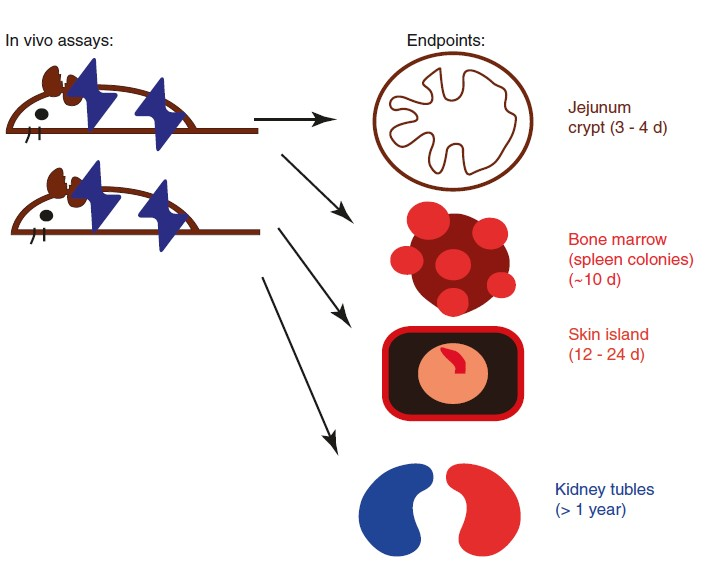
\includegraphics[width=0.8\textwidth]{Imagens/ensaioInVido.jpg}
		}%
		\caption{Ensaios de tecido normal animal. O tempo que leva após a irradiação para observar cada ponto final depende se é um tecido de resposta precoce ou tardia.}
		\label{fig:ensaioInVido}
	\end{figure}

	O ensaio de células-tronco da cripta jejunal é realizado da seguinte maneira:

	\begin{enumerate}[label=\textcolor{CarnationPink}{\arabic*${}^\circ $}]
		\item \textcolor{DarkTurquoise}{\textbf{Preparação do animal:}} nimais de laboratório, como camundongos, são utilizados para realizar o ensaio. Antes do procedimento, os animais são tratados de acordo com os regulamentos éticos e de bem-estar animal.
		\item \textcolor{DarkTurquoise}{\textbf{Preparação do rótulo de marcação:}} Um rótulo de marcação é preparado para acompanhar as células-tronco intestinais. Isso envolve a administração de uma substância que pode ser incorporada nas células-tronco, como bromodeoxiuridina (BrdU), Edu (5-ethynyl-2'-deoxyuridine) ou outros marcadores.
		\item \textcolor{DarkTurquoise}{\textbf{Administração do rótulo de marcação:}} O rótulo de marcação é administrado aos animais, seja por meio de injeção intraperitoneal, administração oral ou outros métodos adequados. A substância de marcação é absorvida e incorporada nas células-tronco intestinais.
		\item \textcolor{DarkTurquoise}{\textbf{Lesão intestinal:}} Após a administração do rótulo de marcação, é induzida uma lesão no tecido intestinal. Isso pode ser feito por meio de agentes químicos, radiação, cirurgia ou outras técnicas que causem danos nas criptas intestinais. No contexto da radiação, os intestinos do camundongo são irradiados com dose suficiente (≥11 Gy) para destruir as vilosidades.
		\item \textcolor{DarkTurquoise}{\textbf{Período de regeneração:}} Após a lesão, o tecido intestinal é deixado para se regenerar por um período de tempo determinado. Durante esse período, as células-tronco intestinais que sobreviveram à lesão e se dividiram podem formar novas criptas. Após 3,5 dias, algumas das criptas jejunais começarão a se regenerar de modo que 1 cripta em regeneração = 1 célula clonogênica sobrevivente.
		\item \textcolor{DarkTurquoise}{\textbf{Preparação e análise do tecido:}} Ao final do período de regeneração, o tecido intestinal é coletado e preparado para análise. Isso pode envolver a fixação, seccionamento e coloração do tecido para permitir a identificação das criptas intestinais.
		\item \textcolor{DarkTurquoise}{\textbf{Avaliação das criptas intestinais:}} As criptas intestinais são avaliadas microscopicamente para contar e analisar as criptas marcadas com o rótulo de marcação. Isso permite determinar a capacidade das células-tronco intestinais de formar novas criptas e regenerar o tecido intestinal.
	\end{enumerate}

	O \textcolor{MediumOrchid}{\textbf{\textit{ensaio de células-tronco da medula óssea}}}, desenvolvido por James Till e Ernest McCulloch, é um ensaio in vivo utilizado para identificar e quantificar células-tronco hematopoiéticas presentes na medula óssea. Nesse ensaio, as células da medula óssea são injetadas em camundongos irradiados ou imunossuprimidos, e a capacidade dessas células de formar colônias de células sanguíneas é avaliada. Esse ensaio foi pioneiro na demonstração da existência de células-tronco hematopoiéticas.

	O \textcolor{MediumOrchid}{\textbf{\textit{ensaio de clone de pele}}} é um ensaio in vivo utilizado para avaliar a presença e a capacidade de regeneração de células-tronco da pele. Nesse ensaio, uma pequena quantidade de células da pele é injetada em uma região da pele de um receptor imunodeficiente, e a capacidade dessas células de formar uma estrutura semelhante a uma epiderme é avaliada. Esse ensaio é utilizado para estudar as células-tronco da pele e a regeneração cutânea.

	O \textcolor{MediumOrchid}{\textbf{\textit{ensaio de túbulos renais}}} é um ensaio in vitro utilizado para avaliar a capacidade de células renais, incluindo células-tronco renais, de formar estruturas semelhantes a túbulos renais funcionais. Nesse ensaio, as células renais são isoladas e cultivadas em condições específicas que promovem a formação de estruturas tridimensionais semelhantes a túbulos renais. A formação dessas estruturas é então avaliada microscopicamente, juntamente com a expressão de marcadores específicos de células renais. Esse ensaio é utilizado para estudar a regeneração renal e a função das células-tronco renais.


\bibliography{ref.bib}
\end{document}